\documentclass[tikz, border=10pt]{standalone}

% Required packages
\usepackage[utf8]{inputenc}
\usepackage[T1]{fontenc}
\usepackage{lmodern} % For smooth fonts
\usepackage{amsmath} % For math symbols like \exists, \in, \land, \notin
\usepackage{tikz}

% TikZ libraries for advanced features
\usetikzlibrary{
    positioning,      % For placing nodes relative to each other (e.g., right=of)
    decorations.pathreplacing, % For drawing curly braces
    arrows.meta,      % For modern arrow tips (e.g., Stealth)
    calc              % For calculating coordinates (e.g., midpoints)
}

\begin{document}
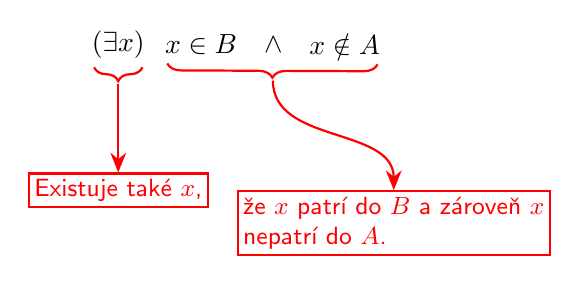
\begin{tikzpicture}[
    % Global style settings
    node distance=0.8em and 1.5em, % Default vertical and horizontal spacing for nodes
    % Style for the red elements
    red_style/.style={
        color=red, 
        thick
    },
    % Style for arrowheads
    arrow_tip/.style={
        -{Stealth[length=2.5mm, width=2mm]}
    },
    % Style for the text labels (smaller font, boxed)
    label_style/.style={
        draw, % This adds the box around the node
        font=\sffamily\small, % Use a small, sans-serif font
        inner sep=2pt, % Add a little padding inside the box
        align=left % Align text to the left for multi-line boxes
    }
]
    % 1. Define the nodes for the main formula.
    \node[inner sep=1pt] (exists_x) {$(\exists x)$};
    \node[inner sep=1pt, right=0.5em of exists_x] (x_in_B) {$x \in B$};
    \node[right=0.5em of x_in_B] (and_op) {$\land$};
    \node[inner sep=1pt, right=0.5em of and_op] (x_not_in_A) {$x \notin A$};

    % 2. Place the two annotation text nodes.
    % We place the first label, then the second one relative to the first to ensure they don't overlap.
    \node[red_style, label_style, below=4em of exists_x] (explanation_part1) {Existuje také $x$,};
    \node[red_style, label_style, right=1em of explanation_part1, anchor=north west] (explanation_part2) {že $x$ patrí do $B$ a zároveň $x$ \\ nepatrí do $A$.};

    % 3. Draw the decorative curly braces (all red, pointing upwards, with small gap).
    \draw[red_style, decorate, decoration={brace, amplitude=5pt, mirror, raise=2pt}]
        ([xshift=2pt]exists_x.south west) -- ([xshift=-2pt]exists_x.south east);
    
    \draw[red_style, decorate, decoration={brace, amplitude=5pt, mirror, raise=2pt}]
        ([xshift=2pt]x_in_B.south west) -- ([xshift=-2pt]x_not_in_A.south east);

    % 4. Draw the arrows, retargeted to the new labels.
    \draw[red_style, arrow_tip] ($(exists_x.south)-(0,8pt)$) to[out=-90, in=90] (explanation_part1.north);
    
    % Define a midpoint for the second part of the formula for the arrow start.
    \coordinate (conjunction_midpoint) at ($(x_in_B.south)!0.5!(x_not_in_A.south)$);
    \draw[red_style, arrow_tip] ($(conjunction_midpoint)-(0,8pt)$) to[out=-90, in=90] (explanation_part2.north);

\end{tikzpicture}
\end{document}
